\chapter{Sperimentazione di seL4}
SeL4 è un sistema open-source dunque lo step successivo è stato quello di scaricare seL4 e sperimentare con mano le funzionalità, ovviamente questo ha richiesto un approfondimento più tecnico e specifico, rispetto a quanto fatto finora, di alcuni aspetti come la gestione della memoria fisica e virtuale, l'IPC ecc. che verranno trattati in questo capitolo.

\section{Prerequisiti}
Come prima cosa ho installato sul mio portatile VirtualBox in quanto come consigliato dalle guide fornite da TS sarebbe ottimale lavorare in ambiente Linux. Non avendo una partizione del portatile con Linux ho inizialmente pensato di utilizzare una macchina virtuale così da lasciare inalterato il mio computer e comunque avere a disposizione un sistema operativo Linux su cui lavorare. Andando avanti con il \textit{set-up} del sistema per iniziare a lavorare su seL4 però ho incontrato una prima difficoltà. Purtroppo lo spazio nel portatile non era tantissimo e la macchina virtuale, considerando il sistema operativo e l'installazione dei vari prerequisiti per poter far girare il \textit{microkernel}, cominciava ad occupare una quantità non trascurabile di GB. Dunque ho dovuto cercare un'alternativa. Per sopperire al problema mi sono procurato un SSD su cui sono andato a copiare la partizione creata in VirtualBox continuando la sperimentazione sul \textit{microkernel} lavorando sull'SSD esterno collegato via USB.

Per lavorare su seL4 è necessario avere installato sul sistema dei programmi che simulino un'architettura su cui farlo eseguire. Per fare ciò è necessario installare delle dipendenze (prerequisiti) cioè compilatori, emulatori software vari e librerie affinché sia possibile utilizzare seL4.\\
Prima di tutto ho installato Google repo, così da poter clonare i repository git:
\definecolor{codegreen}{rgb}{0,0.6,0}
\definecolor{codegray}{rgb}{0.5,0.5,0.5}
\definecolor{codepurple}{rgb}{0.58,0,0.82}
\definecolor{backcolour}{rgb}{0.95,0.95,0.92}
\lstdefinestyle{mystyle}{
    backgroundcolor=\color{backcolour},   
    commentstyle=\color{codegreen},
    keywordstyle=\color{magenta},
    numberstyle=\tiny\color{codegray},
    stringstyle=\color{codepurple},
    basicstyle=\ttfamily\footnotesize,
    breakatwhitespace=false,         
    breaklines=true,                 
    captionpos=b,                    
    keepspaces=true,                  
    numbersep=5pt,                  
    showspaces=false,                
    showstringspaces=false,
    showtabs=false,                  
    tabsize=2
}

\lstset{style=mystyle}

\begin{lstlisting}[language=bash]
sudo apt-get install repo
\end{lstlisting}

build-essential, cmake, ninja, curl, python e QEMU abbreviazione di \textit{Quick EMUlator}, un emulatore \textit{open-source} che permette di emulare un'architettura informatica e quindi diversi sistemi operativi; in questo caso è fondamentale perchè permette l'esecuzione di seL4:
\begin{lstlisting}[language=bash]
sudo apt-get install build-essential
sudo apt-get install cmake ccache ninja-build cmake-curses-gui
sudo apt-get install libxml2-utils ncurses-dev
sudo apt-get install curl git doxygen device-tree-compiler
sudo apt-get install u-boot-tools
sudo apt-get install python3-dev python3-pip python-is-python3
sudo apt-get install protobuf-compiler python3-protobuf
sudo apt-get install qemu-system-arm qemu-system-x86 qemu-system-misc
pip3 install --user setuptools
pip3 install --user sel4-deps
\end{lstlisting}

Altro componente fondamentale è CAmkES (\textit{component architecture for \textit{microkernel}-based embedded systems}), un \textit{framework} per realizzare velocemente sistemi multiserver affidabili basati su \textit{microkernel}
\begin{lstlisting}[language=bash]
pip3 install --user camkes-deps
curl -sSL https://get.haskellstack.org/ | sh
sudo apt-get install haskell-stack
sudo apt-get install clang gdb
sudo apt-get install libssl-dev libclang-dev libcunit1-dev libsqlite3-dev
sudo apt-get install qemu-kvm
\end{lstlisting}

Dopodiché sono passato alle dipendenze per l'installazione di Isabelle (\textit{theorem prover}) che serve per la verifica automatica di sistemi software e hardware:
\begin{lstlisting}[language=bash]
sudo apt-get install \
    python3 python3-pip python3-dev \
    gcc-arm-none-eabi build-essential libxml2-utils ccache \
    ncurses-dev librsvg2-bin device-tree-compiler cmake \
    ninja-build curl zlib1g-dev texlive-fonts-recommended \
    texlive-latex-extra texlive-metapost texlive-bibtex-extra \
    mlton-compiler haskell-stack repo
\end{lstlisting}

Ancora dipendenze Python e Haskell
\begin{lstlisting}[language=bash]
pip3 install --user --upgrade pip
pip3 install --user sel4-deps

stack upgrade --binary-only
which stack # should be $HOME/.local/bin/stack
stack install cabal-install
\end{lstlisting}

Con questa serie di comandi \textit{bash} il sistema operativo Linux, per la precisione Ubuntu 22.04.2 LTS, ha tutti i prerequisiti necessari per procedere alla configurazione.

\section{Configurazione}
Lo step successivo è stato quello di recuperare, attraverso \texttt{repo}, la collezione di \textit{repository} necessari per la verifica di seL4 contenente in particolare, il sorgente del kernel, i \textit{theorem prover} Isabelle/HOL e HOL4 e lo strumento di verifica binaria.
\begin{lstlisting}[language=bash]
mkdir verification
cd verification
repo init -u https://git@github.com/seL4/verification-manifest.git
repo sync
\end{lstlisting}

A questo punto  si avrà quindi una cartella con questa struttura:
\dirtree{%
.1 verification.
.2 HOL4/.
.2 graph-refine/.
.2 isabelle/.
.2 l4v/.
.2 seL4/.
}
Il che indica che l'importazione delle \textit{repository} è andata a buon fine, quindi possiamo procedere alla configurazione di Isabelle posizionandoci nella cartella \texttt{l4v}:
\begin{lstlisting}[language=bash]
mkdir -p ~/.isabelle/etc
cp -i misc/etc/settings ~/.isabelle/etc/settings
./isabelle/bin/isabelle components -a
./isabelle/bin/isabelle jedit -bf
./isabelle/bin/isabelle build -bv HOL
\end{lstlisting}

Questa serie di comandi bash daranno come risultato:
\begin{itemize}
	\item la creazione di una cartella per le impostazioni utente di Isabelle;
	\item l'installazione delle impostazione Isabelle per L4.verified \cite{l4v} il quale è un repository che contiene formalismi per la verifica di seL4;
	\item il download di Scala, Java JDK, PolyML ed altri dimostratori (\textit{prover}) esterni;
	\item la compilazione del Prover IDE (PIDE) jEdit di Isabelle.
\end{itemize} 

\section{Avvio di SeL4}
Terminata la prima fase di installazione dei prerequisiti e di configurazione mi sono procurato ciò che servirà poi per eseguire i test delle varie funzionalità di seL4:
\begin{lstlisting}[language=bash]
mkdir seL4test
cd seL4test
repo init -u https://github.com/seL4/sel4test-manifest.git
repo sync
\end{lstlisting}

Con questi comandi si va a creare una directory \texttt{seL4test} al cui interno ci saranno tutte le direttive e le librerie necessarie per eseguire i vari test e scaricare anche il kernel stesso, attraverso il comando \texttt{repo}.

Successivamente è stato necessario creare una cartella \texttt{build-x86} di configurazione per QEMU in modo da indicargli il \textit{target} su cui eseguire le simulazioni:
\begin{lstlisting}[language=bash]
mkdir build-x86
cd build-x86
../init-build.sh -DPLATFORM=x86_64 -DSIMULATION=TRUE
ninja
\end{lstlisting}

Il comando \texttt{ninja}, che si vedrà spesso a seguire, è un \textit{assembler} che permette di fare il \textit{build} di sistemi anche complessi molto velocemente.

A questo punto è possibile eseguire il comando \texttt{./simulate} che farà partire la simulazione e dopo una lunga serie di test (IPC, chiamate di sistema, thread...) che appariranno nel terminale, concluderà, se tutto è andato a buon fine, con:\\
\texttt{All is well in the universe}\\
Il che indica che seL4 può essere utilizzato in questo ambiente simulato come mostrato in Figura~\ref{fig:Prima simulazione}.
\begin{figure}[H]
  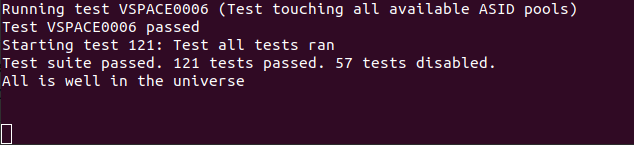
\includegraphics[width=\linewidth]{img/PrimaSimulazione.png}
  \label{fig:Prima simulazione}
\end{figure}

\section{Programmazione con le API livello kernel di seL4}
Una volta procurati tutti i prerequisiti necessari e appurato che seL4 può essere eseguito senza problemi possiamo iniziare a prendere familiarità con il sistema seguendo dei tutorial forniti dalla \textit{seL4 Foundation} \cite{seL4Tutorial}. Tali tutorial contengono programmi semicompleti creati appositamente per sperimentare e far comprendere le funzionalità del sistema, in particolare con le API di seL4 \cite{sel4API}.\\
Come ormai già visto più volte sopra ho recuperato l'ambiente per eseguire i tutorial attraverso l'uso di \texttt{repo}:
\begin{lstlisting}[language=bash]
mkdir sel4-tutorials-manifest
cd sel4-tutorials-manifest
repo init -u https://github.com/seL4/sel4-tutorials-manifest
repo sync
\end{lstlisting}
Ogni tutorial ha un suo \textit{repository} da importare nell'ambiente di lavoro nel quale, tra gli altri file e cartelle, c'è (solitamente) un \texttt{main.c} che sarà quello su cui andare a fare le modifiche per completare il tutorial.

\subsection{Capability}
Prima di tutti ho fatto un approfondimento sulle capability. Come già detto nel capitolo precedente, una capability è un \textit{token} unico che dà accesso ad un'entità del sistema, un puntatore con dei diritti di accesso. In seL4 ci sono 3 tipi di capability:
\begin{enumerate}
	\item capability che controllano l'accesso ad entità del kernel come i thread control block (TCB);
	\item capability che controllano l'accesso a risorse astratte tipo gli interrupt;
	\item untyped capability che sono responsabili della gestione della memoria.
\end{enumerate}

Tutte le capability delle risorse del kernel sono date dal processo \textit{root} all'inizializzazione del sistema, un po' come il processo \texttt{init} nei sistemi unix che è padre di tutti i processi. Quando parliamo di capability ci sono 3 termini fondamentali: CNode, CSlot e CSpace. Il primo di questi è l'abbreviazione di \textit{Capability-Node} ed è un oggetto che contiene delle capability, possiamo pensarlo come un vettore (\textit{array}) di capability. Ogni elemento dell'array è chiamato CSlot (\textit{Capability-Slot}) il quale può avere due stati: \texttt{empty} o \texttt{full}. Ciò equivale, rispettivamente, che il CNode ha una capability nulla oppure una capability ad una risorsa del \textit{kernel}. Per convenzione il primo CSlot, cioè quello situato alla posizione 0 del vettore, è nullo. Invece un CSpace (\textit{Capability-Space}) è il range completo di capability accessibili da un \textit{thread}, che può essere composto da uno o più CNode.

Per fare riferimento ad una capability ed eseguire operazioni su di essa è necessario fare un \texttt{address} (indirizzamento) della capability. Per farlo ci sono due modi in seL4: tramite \textit{invocazione} o con \textit{indirizzamento diretto}.

Per quanto riguarda l'invocazione, ogni \textit{thread} ha uno speciale CNode installato nel suo TCB noto come \texttt{CSpace root}. Questo può essere nullo, ad esempio quando il thread non è autorizzato a invocare nessuna capability, o può avere una capability ad un noto CNode. Quando si vuole fare un \textit{addressing} di una capability attraverso invocazione, un CSlot viene indirizzato implicitamente invocando il CSpace \textit{root} del \textit{thread} che sta facendo l'invocazione.

Per quanto riguarda il metodo dell'indirizzamento diretto invece permette di specificare il CNode piuttosto che utilizzare implicitamente il CSpace \textit{root}. Questo tipo di \textit{addressing}  è usato principalmente per costruire e manipolare i CSpace, potenzialmente il CSpace di un altro \textit{thread}.

L'esercizio proposto in questa sezione è un programma in linguaggio C con una serie di errori da risolvere, il primo tra questi è nel settaggio del numero di \textit{byte} del CNode:
\begin{lstlisting}[language=C++]
int main(int argc, char *argv[]) {

    /* parse the location of the seL4_BootInfo data structure from
    the environment variables set up by the default crt0.S */
    seL4_BootInfo *info = platsupport_get_bootinfo();

    size_t initial_cnode_object_size = BIT(info->initThreadCNodeSizeBits);
    printf("Initial CNode is %zu slots in size\n", initial_cnode_object_size);
    size_t initial_cnode_object_size_bytes = 0; // TODO
    printf("The CNode is %zu bytes in size\n", 	initial_cnode_object_size_bytes);
\end{lstlisting}

Chiaramente \texttt{initial\_cnode\_object\_size\_bytes} non può essere 0, il suo valore invece sarà dato dal numero degli slot del CNode moltiplicato per le dimensione in bit di ognuno di essi:\texttt{initial\_cnode\_object\_size * (1u << seL4\_SlotBits)}.

Eseguendo nuovamente il codice questo darà l'errore \texttt{Attempted to invoke a null cap}. Ciò accade perché il codice cerca di impostare la priorità del TCB del \textit{thread} invocando l'ultimo CSlot del CSpace che però è vuoto.
\begin{lstlisting}[language=C++]
seL4_CPtr first_free_slot = info->empty.start;
seL4_Error error = seL4_CNode_Copy(seL4_CapInitThreadCNode, first_free_slot, seL4_WordBits, seL4_CapInitThreadCNode, seL4_CapInitThreadTCB, seL4_WordBits, seL4_AllRights);
ZF_LOGF_IF(error, "Failed to copy cap!");
%seL4_CPtr last_slot = info->empty.end - 1;
// TODO

/* set the priority of the root task */
error = seL4_TCB_SetPriority(last_slot, last_slot, 10);
ZF_LOGF_IF(error, "Failed to set priority");
\end{lstlisting}

Dunque per risolvere il problema è necessario fare un'altra copia della capability del TCB dentro l'ultimo slot del CNode: per fare ciò utilizziamo \texttt{seL4\_CNode\_Copy} che prende come parametri \texttt{destination root, slot, depth, source root, slot, depth, rights}, dove \texttt{depth} indica quanto bisogna attraversare il CNode per arrivare al CSlot e \texttt{rights} sono invece i diritti ereditati dalla nuova capability; \texttt{first\_free\_slot} è lo slot in cui è stata fatta una copia della capability del TCB del \textit{thread} iniziale qualche riga di codice sopra.
\begin{lstlisting}[language=C++]
seL4_CNode_Copy(seL4_CapInitThreadCNode, last_slot, seL4_WordBits, seL4_CapInitThreadCNode, first_free_slot, seL4_WordBits, seL4_AllRights);
\end{lstlisting}

Rieseguendo il programma non viene più mostrato l'errore predente ma c'è comunque un altro errore \texttt{first\_free\_slot is not empty}. Questo avviene perchè il codice cerca di spostare \texttt{first\_free\_slot} e \texttt{last\_slot} in se stesso, ciò non è possibile (perché è già presente una capability, cioè se stessa) ed è in realtà un escamotage per controllare se un CSlot è vuoto.
\begin{lstlisting}[language=C++]
// TODO 
         
// check first_free_slot is empty
error = seL4_CNode_Move(seL4_CapInitThreadCNode, first_free_slot, seL4_WordBits, seL4_CapInitThreadCNode, first_free_slot, seL4_WordBits);
ZF_LOGF_IF(error != seL4_FailedLookup, "first_free_slot is not empty");

// check last_slot is empty
error = seL4_CNode_Move(seL4_CapInitThreadCNode, last_slot, seL4_WordBits, seL4_CapInitThreadCNode, last_slot, seL4_WordBits);
ZF_LOGF_IF(error != seL4_FailedLookup, "last_slot is not empty");
\end{lstlisting}

Quindi per risolvere il problema è necessario eliminare le due capability. Questo può essere fatto in due modi: eliminando le due copie delle capability usando \texttt{seL4\_CNode\_Delete} oppure con \texttt{seL4\_CNode\_Revoke} sulla capability originale da cui sono state fatte le copie, quest'ultima API elimina tutte le capability figlie di essa. Per fare più velocemente utilizzeremo il secondo metodo che richiede come parametri il CNode e la posizione dentro di esso in cui andare a recuperare la capability (\texttt{CNode, index, depth}):
\begin{lstlisting}[language=C++]
seL4_CNode_Revoke(seL4_CapInitThreadCNode, seL4_CapInitThreadTCB, seL4_WordBits);
\end{lstlisting}

L'esercitazione si conclude con la sospensione del \textit{thread} corrente:
\begin{lstlisting}[language=C++]
seL4_TCB_Suspend(seL4_CapInitThreadTCB);
\end{lstlisting}
Il codice completo del tutorial è riportato in \cite{capability}.

\subsection{Gestione delle memoria}
Nella sezione precedente sono stati elencati i tipi di capability presenti in seL4, al terzo posto nell'elenco troviamo le \texttt{untyped capability}, queste sono il modo con il quale è possibile gestire la memoria fisica nel \textit{microkernel} seL4.

Ad accezione di una piccola parte di memoria del \textit{kernel} tutta la restante è gestita a livello utente. Le capability a tutta la memoria fisica disponibile vengono passate al processo \textit{root} come capability alla \textit{untyped memory}, che non è altro che un blocco contiguo di memoria fisica con una dimensione ben specifica. Per riassumere, in seL4 avremo quindi le \textit{untyped capability} che sono capability alla \textit{untyped memory}. Inoltre le \textit{untyped capability} possono essere riscritte in oggetti del \textit{kernel} insieme alla capability oppure in ulteriori \textit{untyped capability} più piccole.

Le untyped capability hanno anche un flag booleano \textit{device} che indica se la memoria è scrivibile dal \textit{kernel} oppure no: può essere in un'area non accessibile dal \textit{kernel} o riservata ad altri dispositivi.

In seL4 esiste un unico modo per invocare una \textit{untyped capability} cioè attraverso l'utilizzo dell'API \texttt{seL4\_Untyped\_Retype} che serve per creare una nuova \textit{capability} da una \textit{untyped capability}. Nello specifico, questo \textit{retype} darà accesso a un sottoinsieme della memoria della capability di origine che può essere una \textit{untyped capability} più piccola o può puntare ad un nuovo oggetto con un tipo specifico.
\begin{lstlisting}[language=C++]
seL4_Untyped_Retype(parent_untyped, // the untyped capability to retype
                    seL4_UntypedObject, // type
                    untyped_size_bits,  //size
                    seL4_CapInitThreadCNode, // root
                    0, // node_index
                    0, // node_depth
                    child_untyped, // node_offset
                    1); // num_caps
\end{lstlisting}

Le \textit{untyped capability} sono ritipate in maniera incrementale seguendo una politica \textit{greedy} a partire dall'\textit{untyped} invocato. Ogni \textit{untyped capability} mantiene un singolo \textit{watermark}, con gli indirizzi prima di esso non disponibili e quelli successivi liberi. La memoria non può essere liberata fino a che tutti i figli non vengono revocati, dove i figli non sono altro che le nuove capability che vengono create da una \textit{untyped capability}.

Come per la sezione sopra anche qui c'è un \textit{repository} da scaricare con all'interno un file\texttt{ main.c}, che una volta compilato e avviato, stampa a video una lista di tutte le \textit{untyped capability} fornite dal processo \textit{root} all'avvio e segnala un errore \texttt{Untyped Retype: Requested UntypedItem size too small}. Ciò succede perché il programma sta tentando di creare una \textit{untyped} di dimensione 0.
\begin{lstlisting}[language=C++]
int main(int argc, char *argv[]) {
    /* parse the location of the seL4_BootInfo data structure from
    the environment variables set up by the default crt0.S */
    seL4_BootInfo *info = platsupport_get_bootinfo();


    printf("    CSlot   \tPaddr           \tSize\tType\n");
    for (seL4_CPtr slot = info->untyped.start; slot != info->untyped.end; slot++) {
        seL4_UntypedDesc *desc = &info->untypedList[slot - info->untyped.start];
        printf("%8p\t%16p\t2^%d\t%s\n", (void *) slot, (void *) desc->paddr, desc->sizeBits, desc->isDevice ? "device untyped" : "untyped");
    }
    seL4_Error error;

    // list of general seL4 objects
    seL4_Word objects[] = {seL4_TCBObject, seL4_EndpointObject, seL4_NotificationObject};
    // list of general seL4 object size_bits
    seL4_Word sizes[] = {seL4_TCBBits, seL4_EndpointBits, seL4_NotificationBits};
    
    // TODO
    seL4_Word untyped_size_bits = 0; //ERRORE GENERATO QUI
    seL4_CPtr parent_untyped = 0;
    seL4_CPtr child_untyped = info->empty.start;

    // First, find an untyped big enough to fit all of our objects
    for (int i = 0; i < (info->untyped.end - info->untyped.start); i++) {
        if (info->untypedList[i].sizeBits >= untyped_size_bits && !info->untypedList[i].isDevice) {
            parent_untyped = info->untyped.start + i;
            break;
        }
    }
\end{lstlisting}

Per risolvere questo problema è necessario assegnare una dimensione consona alla variabile \texttt{untyped\_size\_bits}. Dato che poi dobbiamo creare uno spazio per tutti gli elementi di \texttt{objects[]} e considerato che la somma di \texttt{seL4\_EndpointBits} e \texttt{seL4\_NotificationBits} è inferiore a \texttt{seL4\_TCBBits} possiamo attribuire alla variabile il valore \texttt{seL4\_TCBBits + 1}. Il +1 fa raddoppiare il numero di \textit{byte} visto che lo spazio assegnato sarà $ 2^{seL4\_TCBBits + 1} $ bit, i quali sono sufficienti per contenere tutti e tre gli elementi.

Eseguendo di nuovo il programma questo procederà fino a che non segnalerà un ulteriore errore \texttt{Failed to set priority}.
\begin{lstlisting}[language=C++]
// create an untyped big enough to retype all of the above objects from
error = seL4_Untyped_Retype(parent_untyped, seL4_UntypedObject, untyped_size_bits, seL4_CapInitThreadCNode, 0, 0, child_untyped, 1);
ZF_LOGF_IF(error != seL4_NoError, "Failed to retype");

// use the slot after child_untyped for the new TCB cap:
seL4_CPtr child_tcb = child_untyped + 1;
// TODO

// try to set the TCB priority
error = seL4_TCB_SetPriority(child_tcb, seL4_CapInitThreadTCB, 10);
ZF_LOGF_IF(error != seL4_NoError, "Failed to set priority");
\end{lstlisting}

L'errore viene generato perché \texttt{child\_tcb} è un CSlot vuoto. Per risolvere è sufficiente assegnare al CSlot una capability creando un \textit{TCB object} da \texttt{child\_untyped}.
\begin{lstlisting}[language=C++]
seL4_Untyped_Retype(child_untyped, seL4_TCBObject, 0, seL4_CapInitThreadCNode, 0, 0, child_tcb, 1);
\end{lstlisting}

Con questa linea di codice il problema è risolto ma l'esecuzione viene bloccata da un altro errore \texttt{Endpoint cap is null cap}.
\begin{lstlisting}[language=C++]
// use the slot after child_tcb for the new endpoint cap:
seL4_CPtr child_ep = child_tcb + 1;
// TODO

// identify the type of child_ep
uint32_t cap_id = seL4_DebugCapIdentify(child_ep);
ZF_LOGF_IF(cap_id == 0, "Endpoint cap is null cap");
\end{lstlisting}

Tale errore è molto simile al precedente: si sta cercando di identificare un \textit{endpoint} nullo. Quindi per risolvere il problema è necessario creare un \textit{endpoint object} sempre da \texttt{child\_untyped} e mettere la capability nel CSlot \texttt{child\_ep}
\begin{lstlisting}[language=C++]
seL4_Untyped_Retype(child_untyped, seL4_EndpointObject, 0, seL4_CapInitThreadCNode, 0, 0, child_ep, 1);
\end{lstlisting}

Alla fine il programma tenta di allocare tutto il \texttt{child\_untyped} come \textit{endpoint} ma fallisce perché tutto lo spazio è stato consumato dalle allocazioni fatte precedentemente. La soluzione al problema è fare una \texttt{seL4\_CNode\_Revoke} (vista sopra) su di esso in modo che tutto le spazio venga liberato e così facendo il programma termina con successo. 
\begin{lstlisting}[language=C++]
// revoke the child untyped
error = seL4_CNode_Revoke(seL4_CapInitThreadCNode, child_untyped, seL4_WordBits);

// allocate the whole child_untyped as endpoints
// Remember the sizes are exponents, so this computes 2^untyped_size_bits / 2^seL4_EndpointBits:
seL4_Word num_eps = BIT(untyped_size_bits - seL4_EndpointBits);
error = seL4_Untyped_Retype(child_untyped, seL4_EndpointObject, 0, seL4_CapInitThreadCNode, 0, 0, child_tcb, num_eps);
ZF_LOGF_IF(error != seL4_NoError, "Failed to create endpoints.");

printf("Success\n");
\end{lstlisting}
Il codice completo del tutorial è riportato in \cite{untyped}.

\subsection{Virtual memory management}
SeL4 non fornisce strumenti per la gestione della memoria virtuale al di là delle primitive per la gestione dell'hardware. Quindi il servizio di \textit{mapping} della memoria e lo \textit{swapping} deve essere gestito a livello utente che ha tutta la libertà di gestirlo in base alle esigenze del sistema. SeL4 mette dunque a disposizione degli oggetti appositi chiamati \textit{VSpace} (\textit{virtual address space}), simili ai CSpace, che sono composti da oggetti forniti dal kernel che variano in base all'architettura hardware (x86\_64, RISC-V, ARM).

Per mappare le pagine sono necessari degli \textit{intermediate hardware virtual memory objects}, praticamente per mappare una pagina è necessario creare una struttura intermedia che varia in base all'architettura. Ad esempio nei sistemi x86\_64 per mappare una pagina sono necessari questi 3 oggetti: \texttt{seL4\_PDPT, seL4\_PageDirectory, seL4\_PageTable}. 

Le API di seL4 forniscono varie funzioni per la mappatura delle memoria in base all'architettura in cui sta girando seL4. Tutte le funzione di \textit{mapping} prendono 3 argomenti principali:
\begin{itemize}
	\item il VSpace in cui mappare l'oggetto;
	\item l'indirizzo virtuale su cui mappare l'oggetto;
	\item gli attributi della memoria virtuale che dipendono dall'architettura.
\end{itemize}
Un esempio di mappatura di un oggetto \texttt{seL4\_PDPT} ad un certo indirizzo \texttt{TEST\_VADDR} è:
\begin{lstlisting}[language=C++]
seL4_X86_PDPT_Map(pdpt, seL4_CapInitThreadVSpace, TEST_VADDR, seL4_X86_Default_VMAttributes);
\end{lstlisting}

Una volta che le strutture di paginazione intermedie sono state mappate in un certo range di indirizzi virtuali, i \textit{frame} fisici possono essere mappati in quel range attraverso l'invocazione del \textit{frame capability}.\\
Ecco un esempio di mappatura di un frame:
\begin{lstlisting}[language=C++]
seL4_X86_Page_Map(frame, seL4_CapInitThreadVSpace, TEST_VADDR, seL4_CanRead, seL4_X86_Default_VMAttributes);
\end{lstlisting}

Come si vede questo metodo prende un argomento in più perché per mappare i frame vengono richiesti anche i diritti che determineranno il tipo di mappatura (nell'esempio sopra diritti di sola lettura).

Il tutorial di questa sezione fornisce un programma che all'avvio termina con l'errore \texttt{Missing intermediate paging structure at level 30}.
\begin{lstlisting}[language=C++]
int main(int argc, char *argv[]) {
    /* parse the location of the seL4_BootInfo data structure from
    the environment variables set up by the default crt0.S */
    seL4_BootInfo *info = platsupport_get_bootinfo();
    seL4_Error error;
    seL4_CPtr frame = alloc_object(info, seL4_X86_4K, 0);
    seL4_CPtr pdpt = alloc_object(info, seL4_X86_PDPTObject, 0);
    seL4_CPtr pd = alloc_object(info, seL4_X86_PageDirectoryObject, 0);
    seL4_CPtr pt = alloc_object(info, seL4_X86_PageTableObject, 0);

	// TODO
	
	// TODO

    /* map a PDPT at TEST_VADDR */
    error = seL4_X86_PDPT_Map(pdpt, seL4_CapInitThreadVSpace, TEST_VADDR, seL4_X86_Default_VMAttributes);

    /* map a read-only page at TEST_VADDR */
    error = seL4_X86_Page_Map(frame, seL4_CapInitThreadVSpace, TEST_VADDR, seL4_CanRead, seL4_X86_Default_VMAttributes);
    if (error == seL4_FailedLookup) {
        printf("Missing intermediate paging structure at level %lu\n", seL4_MappingFailedLookupLevel());
    }
    ZF_LOGF_IF(error != seL4_NoError, "Failed to map page");
\end{lstlisting}

L'errore è dovuto al fatto che per mappare una pagina tutte le strutture di paginazione intermedie devono essere mappate; il valore \texttt{30} equivale alla costante \texttt{SEL4\_MAPPING\_LOOKUP\_NO\_PD} il che indica che è necessario mappare un oggetto \textit{page directory} che può essere fatto con l'apposito metodo \texttt{seL4\_X86\_PageDirectory\_Map}:
\begin{lstlisting}[language=C++]
seL4_X86_PageDirectory_Map(pd, seL4_CapInitThreadVSpace, TEST_VADDR, seL4_X86_Default_VMAttributes);
\end{lstlisting}

Ricompilando ed eseguendo il codice appare un errore simile al precedente \texttt{Missing intermediate paging structure at level 21} dove il valore \texttt{21} questa volta indica la costante \texttt{SEL4\_MAPPING\_LOOKUP\_NO\_PT} che suggerisce di mappare un oggetto di tipo \textit{page table}
\begin{lstlisting}[language=C++]
seL4_X86_PageTable_Map(pt, seL4_CapInitThreadVSpace, TEST_VADDR, seL4_X86_Default_VMAttributes);
\end{lstlisting}

Adesso il codice procede mappando la pagina però successivamente (come si può leggere nel codice sotto) avviene un tentativo di scrittura sulla pagina che genera un errore perché la pagina era stata mappata in sola lettura \texttt{seL4\_CanRead}. L'errore può dunque essere evitato facendo una rimappatura della pagina, questa volta in lettura e scrittura.
\begin{lstlisting}[language=C++]
seL4_X86_Page_Map(frame, seL4_CapInitThreadVSpace, TEST_VADDR, seL4_ReadWrite, seL4_X86_Default_VMAttributes);
\end{lstlisting}

Il \textit{mapping} delle pagine può anche essere disfatto utilizzando \texttt{unmap} sulla pagina o su qualsiasi struttura intermedia di paginazione; alternativamente può essere fatto eliminando la capability finale di qualsiasi struttura di paginazione.\\
Il codice completo del tutorial è riportato in \cite{mapping}.

\subsection{Thread}
SeL4 per rappresentare l'esecuzione di un processo e gestire i tempi di esecuzione fornisce i \textit{thread}. Essi sono realizzati attraverso \textit{thread control block object} (TCBs) e ce ne sono uno per ogni \textit{thread} del kernel.\\
Come sappiamo in un SO è lo \textit{scheduler} a decidere quale processo e per quanto tempo può utilizzare la CPU. In seL4, come avevamo già visto nel capitolo precedente, la politica di \textit{scheduling} è un integrazione di \textit{round-robin} e \textit{scheduling a priorità}: lo \textit{scheduler} sceglie i \textit{thread} con maggiore priorità che sono pronti e se ce ne sono con la stessa priorità questi saranno scelti in ordine FIFO seconda la politica \textit{round-robin}. La priorità è determinata da un range che va da 0 (\texttt{seL4\_MinPrio}) a 255 (\texttt{seL4\_MaxPrio}). Oltre alla priorità un TCBs contiene anche un \textit{maximum control priority} (MCP) che serve per controllare che un processo non modifichi la priorità di un altro processo (o di se stesso) impostandola più alta della sua. Quindi un processo che vuole modificare una priorità deve fornire la sua capability (di \textit{thread}) in modo da determinare se è autorizzato a impostare quella priorità.

L'esercizio per questa sezione, se fatto partire senza nessuna modifica, inizialmente mostrerà a video una tabella di tutti i TCB (questo è ottenuto tramite una chiamata di sistema di debug \texttt{seL4\_DebugDumpScheduler()}) e successivamente lancia un errore \texttt{Failed to retype thread: 2} come in Figura~\ref{fig:TutorialThreads}.\\
\begin{figure}[h]
  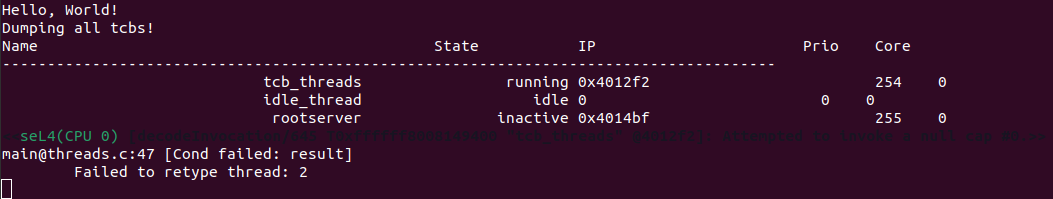
\includegraphics[width=\linewidth]{img/Threads.png}
  \caption{lista TCB}
  \label{fig:TutorialThreads}
\end{figure}

Questo errore avviene perché c'è un errata invocazione del metodo \texttt{seL4\_Untyped\_Retype()}.
\begin{lstlisting}[language=C++]
// the root CNode of the current thread
extern seL4_CPtr root_cnode;
// VSpace of the current thread
extern seL4_CPtr root_vspace;
// TCB of the current thread
extern seL4_CPtr root_tcb;
// Untyped object large enough to create a new TCB object

extern seL4_CPtr tcb_untyped;
extern seL4_CPtr buf2_frame_cap;
extern const char buf2_frame[4096];

// Empty slot for the new TCB object
extern seL4_CPtr tcb_cap_slot;
// Symbol for the IPC buffer mapping in the VSpace, and capability to the mapping
extern seL4_CPtr tcb_ipc_frame;
extern const char thread_ipc_buff_sym[4096];
// Symbol for the top of a 16 * 4KiB stack mapping, and capability to the mapping
extern const char tcb_stack_base[65536];
static const uintptr_t tcb_stack_top = (const uintptr_t)&tcb_stack_base + sizeof(tcb_stack_base);

int new_thread(void *arg1, void *arg2, void *arg3) {
    printf("Hello2: arg1 %p, arg2 %p, arg3 %p\n", arg1, arg2, arg3);
    void (*func)(int) = arg1;
    func(*(int *)arg2);
    while(1);
}

int main(int c, char* arbv[]) {

    printf("Hello, World!\n");

    seL4_DebugDumpScheduler();
	// TODO
    seL4_Error result = seL4_Untyped_Retype(seL4_CapNull, seL4_TCBObject, seL4_TCBBits, seL4_CapNull, 0, 0, seL4_CapNull, 1);
    ZF_LOGF_IF(result, "Failed to retype thread: %d", result);
    seL4_DebugDumpScheduler();
\end{lstlisting}

Come si può vedere, al metodo viene passato un oggetto \texttt{seL4\_CapNull} come oggetto da ritipare che ovviamente genera l'errore. Dunque un modo corretto per sistemare questo errore è utilizzare gli oggetti creati nelle variabili globali del codice.
\begin{lstlisting}[language=C++]
seL4_Error result = seL4_Untyped_Retype(tcb_untyped, seL4_TCBObject, seL4_TCBBits, root_cnode, 0, 0, tcb_cap_slot, 1);
\end{lstlisting}

Rieseguendo il codice vedremo che l'errore è risolto e tra la lista dei TCB adesso è presente anche quello appena creato. Dopo aver risolto questo problema si presenta un errore \texttt{Failed to configure thread: 2} in quanto la configurazione del TCB viene fatta tutta su valori nulli.
\begin{lstlisting}[language=C++]
result = seL4_TCB_Configure(seL4_CapNull, seL4_CapNull, 0, seL4_CapNull, 0, 0, (seL4_Word) NULL, seL4_CapNull);
ZF_LOGF_IF(result, "Failed to configure thread: %d", result);
\end{lstlisting}

Il metodo \texttt{seL4\_TCB\_Configure} prende come parametri:
\begin{lstlisting}[language=C++]
seL4_TCB_Configure(tcb, // tcb su cui operare
					cspace_root, // nuovo CSpace root
					cspace_root_data, // opzionale: setta il nuovo CNode
					vspace_root, // nuovo VSpace root
					vspace_root_data, // non ha effetto su x86 e ARM
					buffer, // locazione dell'IPC buffer
					bufferFrame); // IPC buffer
\end{lstlisting} 

Possiamo quindi procedere alla corretta configurazione del TCB in modo da avere lo stesso CSpace e VSpace del thread corrente.
\begin{lstlisting}[language=C++]
result = seL4_TCB_Configure(tcb_cap_slot, seL4_CapNull, root_cnode, 0, root_vspace, 0, (seL4_Word) thread_ipc_buff_sym, tcb_ipc_frame);
\end{lstlisting}

Adesso l'errore che si presenta sarà un altro
\texttt{Failed to set the priority for the new TCB object} questo perchè la priorità data al thread ha valore 0.
\begin{lstlisting}[language=C++]
result = seL4_TCB_SetPriority(tcb_cap_slot, seL4_CapNull, 0);
ZF_LOGF_IF(result, "Failed to set the priority for the new TCB object.\n");
seL4_DebugDumpScheduler();
\end{lstlisting}

Il \textit{thread} corrente ha un MCP di 254 quindi è possibile assegnare questo valore come priorità. Per poterlo fare è necessario anche cambiare il valore \texttt{seL4\_CapNull} e sostituirlo con il TCB del \textit{thread} corrente \texttt{root\_tcb}.

Dopodiché è necessario impostare in maniera adeguata i registri iniziali, in particolare il \textit{program counter} e lo \textit{stack pointer}. È possibile farlo grazie alle utility contenute in \texttt{libsel4utils}.
\begin{lstlisting}[language=C++]
seL4_UserContext regs = {0};
int error = seL4_TCB_ReadRegisters(tcb_cap_slot, 0, 0, sizeof(regs)/sizeof(seL4_Word), &regs);
ZF_LOGF_IFERR(error, "Failed to read the new thread's register set.\n");

// TODO
sel4utils_set_instruction_pointer(&regs, (seL4_Word)new_thread);
// TODO
sel4utils_set_stack_pointer(&regs, tcb_stack_top);
// TODO
error = seL4_TCB_WriteRegisters(tcb_cap_slot, 0, 0, sizeof(regs)/sizeof(seL4_Word), &regs);
ZF_LOGF_IFERR(error, "Failed to write the new thread's register set.\n"
                  "\tDid you write the correct number of registers? See arg4.\n");
seL4_DebugDumpScheduler();
\end{lstlisting}

A questo punto è possibile far partire il \textit{thread} ma per farlo è necessario fare un piccolo aggiustamento nel codice.
\begin{lstlisting}[language=C++]
//resume the new thread
error = seL4_TCB_Resume(seL4_CapNull);
ZF_LOGF_IFERR(error, "Failed to start new thread.\n");
while(1);
return 0;
}
\end{lstlisting}

Chiaramente il \texttt{seL4\_TCB\_Resume} va fatto sul nostro \texttt{tcb\_cap\_slot} e non su \texttt{seL4\_CapNull}. Ora il nuovo \textit{thread} viene eseguito e mostra a video\\
\texttt{Hello2: arg1 0, arg2 0, arg3 0}
Come si può vedere i valori passati al nuovo \textit{thread} sono tutti 0. Se volessimo passare valori differenti potremmo utilizzare la funzione \texttt{sel4utils\_arch\_init\_local\_context} facendo le dovute modifiche al codice.
\begin{lstlisting}[language=C++]
UNUSED seL4_UserContext regs = {0};
int error = seL4_TCB_ReadRegisters(tcb_cap_slot, 0, 0, sizeof(regs)/sizeof(seL4_Word), &regs);
ZF_LOGF_IFERR(error, "Failed to read the new thread's register set.\n"
              "\tDid you write the correct number of registers? See arg4.\n");

sel4utils_arch_init_local_context((void*)new_thread,
                                  (void *)1, (void *)2, (void *)3,
                                  (void *)tcb_stack_top, &regs);
error = seL4_TCB_WriteRegisters(tcb_cap_slot, 0, 0, sizeof(regs)/sizeof(seL4_Word), &regs);
ZF_LOGF_IFERR(error, "Failed to write the new thread's register set.\n"
              "\tDid you write the correct number of registers? See arg4.\n");
\end{lstlisting}
Il codice completo del tutorial è riportato in \cite{threads}.

\subsection{IPC}
\textit{InterProcess Communication} è il meccanismo che utilizza il \textit{microkernel} per sincronizzare lo scambio di  piccole quantità di dati e capability tra i processi. In seL4 l'IPC è facilitato dal fatto che gli oggetti del \textit{kernel} sono di piccole dimensioni, noti come \textit{endpoint} e fungono da porte per la comunicazione; quindi per mandare e ricevere messaggi IPC bisogna farlo attraverso invocazioni sugli \textit{endpoint}.

I \textit{thread} possono mandare messaggi sugli \textit{endpoint} con la \textit{system call} \texttt{seL4\_Send} che è bloccante, mentre possono usare \texttt{seL4\_Recv} per ricevere messaggi.

\texttt{seL4\_Call} invece è una chiamata di sistema che combina le due precedenti con una differenza: nella fase di ricezione il \textit{thread} che usa questa funzione è bloccato su una \textit{one-time capability} chiamata \textit{reply capability} e non sull'\textit{endpoint} stesso come avverrebbe normalmente con la \texttt{seL4\_Recv}. La \textit{replay capability} è contenuta nel TCB del ricevente.

La \textit{system call} \texttt{seL4\_Reply} invoca la \textit{reply capability} la quale manderà un IPC che farà risvegliare il processo bloccato. \texttt{seL4\_ReplyRecv} fa lo stesso ma invia la risposta e blocca l'\textit{endpoint} fornito in una chiamata di sistema combinata.

Ogni \textit{thread} ha un \textit{buffer} che contiene il \textit{payload} del messaggio IPC composto da dati e capability. Il mittente del messaggio specifica la lunghezza e il \textit{kernel} copia questa quantità tra il mittente e il destinatario dell'\textit{IPC buffer}. Quest'ultimo contiene un'area limitata di registri di messaggio (\textit{message registers} abbreviato MR) che sono utilizzati per trasmettere dati sull'IPC. Ogni registro ha dimensione una parola (\textit{word}) (dimensione relativa alla macchina) e la lunghezza massima di un messaggio è contenuta nella costante \texttt{seL4\_MsgMaxLength}. Per caricare un messaggio dentro il \textit{buffer} è possibile utilizzare \texttt{seL4\_SetMR} mentre per estrarlo \texttt{seL4\_GetMR}; la quantità di parole che possono entrare in un registro è disponibile nelle costante \texttt{seL4\_FastMessageRegisters}.

Insieme al messaggio il \textit{kernel} consegna il \textit{badge} dell'\textit{endpoint capability} sul quale il mittente ha fatto l'invocazione per mandare il messaggio. È possibile assegnare un \textit{badge} all'\textit{endpoint} utilizzando \texttt{seL4\_CNode\_Mint} oppure \texttt{seL4\_CNode\_Mutate}, una volta che è stato messo il \textit{badge} sull'\textit{endpoint} questo viene trasferito a tutti i destinatari che ricevono un messaggio su quell'\textit{endpoint}.

SeL4, per codificare la descrizione di un messaggio IPC, usa la struttura dati \texttt{seL4\_MessageInfo\_t} il quale ha la dimensione di una parola ed è composta dai seguenti campi:
\begin{itemize}
	\item[-] \texttt{length} la quantità di dati nel messaggio;
	\item[-] \texttt{extraCaps} numero di capability nel messaggio;
	\item[-] \texttt{capsUnwrapped} marca le capability unwrapped dal kernel;
	\item[-] \texttt{label} dati che verranno trasferiti che non sono statoi modificati dal kernel.
\end{itemize}

Come già accennato, insieme ai dati, attraverso l'IPC, è possibile scambiare anche capability. In gergo questo viene chiamato \textit{cap transfer}:
\begin{lstlisting}[language=C++]
//Invio di una capability via IPC
seL4_MessageInfo info = seL4_MessageInfo_new(0, 0, 1, 0);
seL4_SetCap(0, free_slot);
seL4_Call(endpoint, info);

//Ricezione di una capability
seL4_SetCapReceivePath(cnode, badged_endpoint, seL4_WordBits);
seL4_Recv(endpoint, &sender);
\end{lstlisting}

Il numero di capability trasferite è codificato nella struttura dati \texttt{seL4\_MessageInfo\_t} come \texttt{extraCaps}.
Inoltre seL4 può fare la cosiddetta \textit{unwrap} (scartare) delle capability sull'IPC: se l'n-esima capability nel messaggio si riferisce all'\textit{endpoint} attraverso il quale il messaggio viene inviato, la capability viene \textit{unwrapped}: il suo badge viene inserito nell'n-esima posizione dell'IPC buffer del destinatario (\texttt{caps\_or\_badges}) e il \textit{kernel} imposta l'n-esimo bit nel campo \texttt{capsUnwrapped} del \texttt{seL4\_MessageInfo\_t}.

L'unico modo che hanno i processi per comunicare, nei sistemi basati su \textit{microkernel}, è attraverso l'utilizzo dell'IPC. Essendo tutti i servizi a livello utente si può intuire che di questa funzionalità ne verrà fatto un utilizzo massiccio. Quindi è necessario che sia ottimizzato al meglio e che magari ci siano scorciatoie per renderlo ancora più efficiente in quanto da esso dipendono le prestazioni dell'intero sistema.

Per soddisfare questa esigenza è stato introdotto il \textit{fastpath}, cioè un cammino nel \textit{kernel} altamente ottimizzato che garantisce velocità nell'IPC. Per potersi definire tale deve soddisfare cinque condizioni:
\begin{itemize}
	\item devono essere usate le \textit{system call} \texttt{seL4\_Call} o \texttt{seL4\_ReplyRecv};
	\item i dati del messaggio devono entrare nel registro \texttt{seL4\_FastMessageRegisters};
	\item i processi devono avere spazi di indirizzi validi;
	\item non dovrebbero essere trasferite capability;
	\item nessun altro \textit{thread} nello \textit{scheduler} con priorità superiore a quello sbloccato dall'IPC può essere in esecuzione.
\end{itemize}

In questa sezione l'esercizio è un po' diverso. Non c'è un unico \textit{file main} in cui è contenuto tutto il codice ma c'è un \texttt{server.c} e due \textit{client} \texttt{client\_1.c} e \texttt{client\_2.c} i quali manderanno dei messaggi al \textit{server} che farà da \textit{echo}; tutti i processi hanno accesso ad un unico \textit{endpoint capability} che fornisce accesso allo stesso \textit{endpoint object}.\\
Al primo avvio si ha questo output:
\begin{figure}[H]
  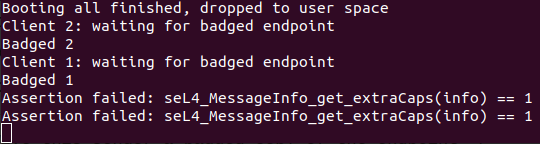
\includegraphics[scale=0.7]{img/PrimoAvvioIPC2.png}%width=\linewidth
  \centering
  \label{fig:PrimoAvvio}
\end{figure}

Gli errori sono dovuti al fatto che entrambi i \textit{client} si mettono in attesa, sull'\textit{endpoint} fornito, di un \textit{badged endpoint} tramite \textit{cap tranfer} che però il \textit{server} non invierà in quanto esso risponde solo ai messaggi dei \textit{client}.
\begin{lstlisting}[language=C++]
// cslot containing IPC endpoint capability
extern seL4_CPtr endpoint;
// cslot containing a capability to the cnode of the server
extern seL4_CPtr cnode;
// empty cslot
extern seL4_CPtr free_slot;

int main(int c, char *argv[]) {

	seL4_Word sender;
    seL4_MessageInfo_t info = seL4_Recv(endpoint, &sender);
    while (1) {
	    seL4_Error error;
        if (sender == 0) {

             /* No badge! give this sender a badged copy of the endpoint */
             seL4_Word badge = seL4_GetMR(0);
             seL4_Error error = seL4_CNode_Mint(cnode, free_slot, seL4_WordBits,
                                                cnode, endpoint, seL4_WordBits,
                                                seL4_AllRights, badge);
             printf("Badged %lu\n", badge);

             // TODO
             
             /* reply to the sender and wait for the next message */
             seL4_Reply(info);

             /* now delete the transferred cap */
             error = seL4_CNode_Delete(cnode, free_slot, seL4_WordBits);
             assert(error == seL4_NoError);

             /* wait for the next message */
             info = seL4_Recv(endpoint, &sender);
\end{lstlisting}

Dunque per risolvere questo problema è necessario impostare il \textit{cap transfer} in modo che i \textit{client} ricevano il \textit{badged endpoint}
\begin{lstlisting}[language=C++]
info = seL4_MessageInfo_new(0, 0, 1, 0);
seL4_SetCap(0, free_slot);
\end{lstlisting}

Compilando e riavviando il programma sembra vada tutto bene eccetto che il sistema si blocca come si vede nella figura sottostante
\begin{figure}[H]
  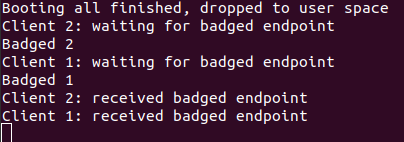
\includegraphics[scale=0.7]{img/DopoBadgeIPC.png}%width=\linewidth
  \centering
  \label{fig:AvvioDopoBadge}
\end{figure}

Ciò succede perché al \textit{server} manca l'implementazione della sua funzione di \textit{echo} dei messaggi che gli vengono inviati; tale funzione può essere fatta scorrendo e stampando a video il contenuto dei \textit{message register}.\\
I \textit{client} mandano rispettivamente le stringhe {"quick", "fox", "over", "lazy"} il \texttt{client\_1} mentre il \texttt{client\_2} {"the", "brown", "jumps", "the", "dog"}.
\begin{lstlisting}[language=C++]
for (int i = 0; i < seL4_MessageInfo_get_length(info); i++) {
printf("%c", (char) seL4_GetMR(i));
}
printf("\n");
\end{lstlisting}

A questo punto però vedremo stampata a video sempre la stessa parola \texttt{the} in \textit{loop} perché il server non manda un \textit{feedback} di risposta al \textit{client} e di conseguenza continua a stampare l'ultima parola ricevuta.
\begin{lstlisting}[language=C++]
for (int i = 0; i < seL4_MessageInfo_get_length(info); i++) {
	printf("%c", (char) seL4_GetMR(i));
}
printf("\n");

// reply to the client and wait for the next message
info = seL4_ReplyRecv(endpoint, info , &sender);
\end{lstlisting}

Rieseguendo, l'output sarà la stampa a video prima di tutte le parole inviate dal \texttt{client\_2} seguite da quelle del \texttt{client\_1}, possiamo modificare il codice in modo da alternare le stampe dei due \textit{client} utilizzando \texttt{seL4\_CNode\_SaveCaller} e \texttt{free\_slot} per salvare le risposte.
\begin{lstlisting}[language=C++]
for (int i = 0; i < seL4_MessageInfo_get_length(info); i++) {
printf("%c", (char) seL4_GetMR(i));
}
printf("\n");

error = seL4_CNode_SaveCaller(cnode, free_slot, seL4_WordBits);
assert(error == 0);
info = seL4_Recv(endpoint, &sender);
for (int i = 0; i < seL4_MessageInfo_get_length(info); i++) {
   printf("%c", (char) seL4_GetMR(i));
}
printf("\n");
seL4_Send(free_slot, seL4_MessageInfo_new(0, 0, 0, 0));

// reply to the client and wait for the next message
info = seL4_ReplyRecv(endpoint, info, &sender);
\end{lstlisting}

Una volta eseguite tutte le correzioni l'\textit{output} finale sarà il seguente:
\begin{lstlisting}[language=bash]
Client 2: received badged endpoint
the
Client 1: received badged endpoint
quick
fox
brown
jumps
over
lazy
the
dog
\end{lstlisting}
Il codice completo del server è riportato in \cite{IPCserver}.\\
Il codice completo del client\_1 è riportato in \cite{IPCclient1}.\\
Il codice completo del client\_2 è riportato in \cite{IPCclient2}.